\documentclass[11pt]{report}
\usepackage[english, german]{babel}
\usepackage{geometry}                % See geometry.pdf to learn the layout options. There are lots.
\geometry{a4paper}                   % ... or a4paper or a5paper or ... 
%\usepackage[parfill]{parskip}    % Activate to begin paragraphs with an empty line rather than an indent
\usepackage{xifthen}
\usepackage{xstring}			% to check content of strings in xifthen
\usepackage{graphicx}
\usepackage[usenames,dvipsnames,table]{xcolor}
\usepackage{amssymb}
\usepackage{epstopdf}
\usepackage[utf8]{inputenc}
\usepackage{hyperref}
\usepackage{fancyhdr}
%\usepackage{natbib}
\usepackage{url}
%for images alignment - added by Nenad
\usepackage[export]{adjustbox}
\usepackage{wrapfig}

\newcommand{\titleofthesis}{Bad-Designer}
\newcommand{\department}{Informatik} % Replace by your department

\newcommand{\firstauthor}{Philipp Auinger}
\newcommand{\firstauthorclass}{5BHIF}
\newcommand{\secondauthor}{Nenad Tripic}
\newcommand{\secondauthorclass}{5BHIF}
%\newcommand{\thirdauthor}{Alfred Wiedermann}
%\newcommand{\thirdauthorclass}{5AHBG}
% \newcommand{\fourthauthor}{Wolfgang Holzer}
% \newcommand{\fourthauthorclass}{5AHEL}

\newcommand{\duedateen}{April 3, 2020} % due date in english format
\newcommand{\duedatede}{3. April 2020} % due date in german format
\newcommand{\supervisor}{Prof. Dipl-Ing. Michael Bucek}
\newcommand{\projectpartner}{Lang+Lang GmbH}
 % Set basic data (author, title, etc.) of your thesis
\IfStrEq*{\languagename}{english}
	{
		\newcommand{\dalabel}{Diploma Thesis}
		\newcommand{\submittedlabel}{Submitted by}
		\newcommand{\datelabel}{Date}
		\newcommand{\duedatevalue}{\duedateen}
		\newcommand{\supervisorlabel}{Supervisor}
		\newcommand{\projectpartnerlabel}{Project Partner}
	}
	{
		\newcommand{\dalabel}{Diplomarbeit}
		\newcommand{\submittedlabel}{Eingereicht von}
		\newcommand{\datelabel}{Datum}
		\newcommand{\duedatevalue}{\duedatede}
		\newcommand{\supervisorlabel}{Betreuer}
		\newcommand{\projectpartnerlabel}{Projektpartner}
	}
 % This file should not really be touched

\begin{document}
\rhead{
\includegraphics[scale=.9]{images/Logo.png}}
\cfoot{}
\begin{titlepage}
\thispagestyle{fancy}

\begin{center}

\vspace*{8em}

{\LARGE \dalabel}

\vspace{2em}

{\large Höhere Technische Bundeslehranstalt Leonding \\[.5em]
Abteilung für \department}

%\vspace{8em}
\vspace*{\fill}

{\Huge \titleofthesis}
\end{center}

%\vspace{8em}
\vspace*{\fill}

\begin{tabular}{ll}
\ifthenelse{\isundefined{\firstauthor}}{}{\submittedlabel: & {\bf \firstauthor, \firstauthorclass}}
\ifthenelse{\isundefined{\secondauthor}}{}{ \\[.5em] & {\bf \secondauthor, \secondauthorclass}}
 \\[.5em]
\datelabel: & {\bf \duedatevalue} \\[.5em]

\supervisorlabel: & {\bf \supervisor} \\[.5em]

\ifthenelse{\isundefined{\projectpartner}}{}{\projectpartnerlabel: & {\bf \projectpartner}}
\end{tabular}
\end{titlepage}
 % Should not be necessary to touch this file
\section*{Eidesstattliche Erklärung}
Hiermit erkläre ich an Eides statt, dass ich die vorgelegte Diplomarbeit selbstständig und ohne Benutzung anderer als der angegebenen Hilfsmittel angefertigt habe. Gedanken, die aus fremden Quellen direkt oder indirekt übernommen wurden, sind als solche gekennzeichnet.

Die Arbeit wurde bisher in gleicher oder ähnlicher Weise keiner anderen Prüfungsbehörde vorgelegt und auch noch nicht veröffentlicht. \\[1em]
Leonding, am \duedatede \\[5em]
\ifthenelse{\isundefined{\firstauthor}}{}{\firstauthor}
\ifthenelse{\isundefined{\secondauthor}}{}{\kern-1ex, \secondauthor} \\[5em]


\begin{otherlanguage}{english}
\section*{Declaration of Academic Honesty}
Hereby, I declare that I have composed the presented paper independently on my own and without any other resources than the ones indicated. All thoughts taken directly or indirectly from external sources are properly denoted as such.

This paper has neither been previously submitted to another authority nor has it been published yet. \\[1em]
Leonding, \duedateen \\[5em]
\ifthenelse{\isundefined{\firstauthor}}{}{\firstauthor}
\ifthenelse{\isundefined{\secondauthor}}{}{\kern-1ex, \secondauthor}
\end{otherlanguage}


\begin{abstract}
	\begin{itemize}
		\item {\em Aufgabenstellung} \\ Um den Kunden der Firma {\projectpartner} die Visualisierung eines für sie designten Bades zu erleichtern, ist es notwendig, ihnen eine möglichst genaue und detaillierte Darstellung anzubieten. Dies bezieht sich sowohl auf das Design, die Komponenten als auch für die Bauanleitung. Da nicht nur die Hotelketten das Modell zu Gesicht bekommen, sondern auch Monteure, die sich daran beim Zusammenbauen orientieren können. Dadurch dass der Fortschritt und das fertige Bad aus verschiedenen Perspektiven angesehen werden kann, wird die Vision für alle klarer und einfacher. Da die ganze Applikation webbasiert ist, ist sie plattformunabhängig und kann dank Electron lokal und ohne Internet ausgeführt werden. Bisher wurde dies immer mit Präsentationsvideos umgesetzt, die jedoch sehr unflexibel sind und zeitintensiv waren. Die Probleme waren dabei, dass das Bad immer nur aus einer Perspektive zu sehen war, das Modell nicht interaktiv war und Kundenwünsche nicht sofort umgesetzt werden konnten. Der Umgang mit dem Tool wird möglichst intuitiv erfolgen und besondere Ressourcenanforderungen sind nicht präsent.
		\item {\em Umsetzung} \\ Die Web-Anwendung basiert auf den gängigen Technologien HTML, JavaScript, Three.js und WEB.GL. Dies ermöglicht es über einen beliebigen Browser und beliebiges Betriebssystem darauf zuzugreifen. Die einzige Anforderung ist eine Internetverbindung. Die Wahl für die oben genannten Technologien ist darauf zurückzuführen, dass alle robust, zukunftssicher, gut dokumentiert und weitverbreitet sind. Damit eignen sie sich perfekt für die Applikation und sind ein wichtiger Beitrag dafür das die Anwendung wartbar ist und bleibt.
		\item {\em Ergebnisse} \\ Die Software wurde nach Abschluss der Arbeit an das Unternehmen {\projectpartner} übergeben. Demonstrationen und Tutorials an die zukünftigen Anwender wurden durch das Entwicklerteam durchgeführt. Unter folgender Adresse \url{http://vm85.htl-leonding.ac.at/} kann die Diplomarbeit begutachtet und verwendet werden.
	\end{itemize}
\clearpage \newpage	
	
\begin{figure}[h]
    \centering
    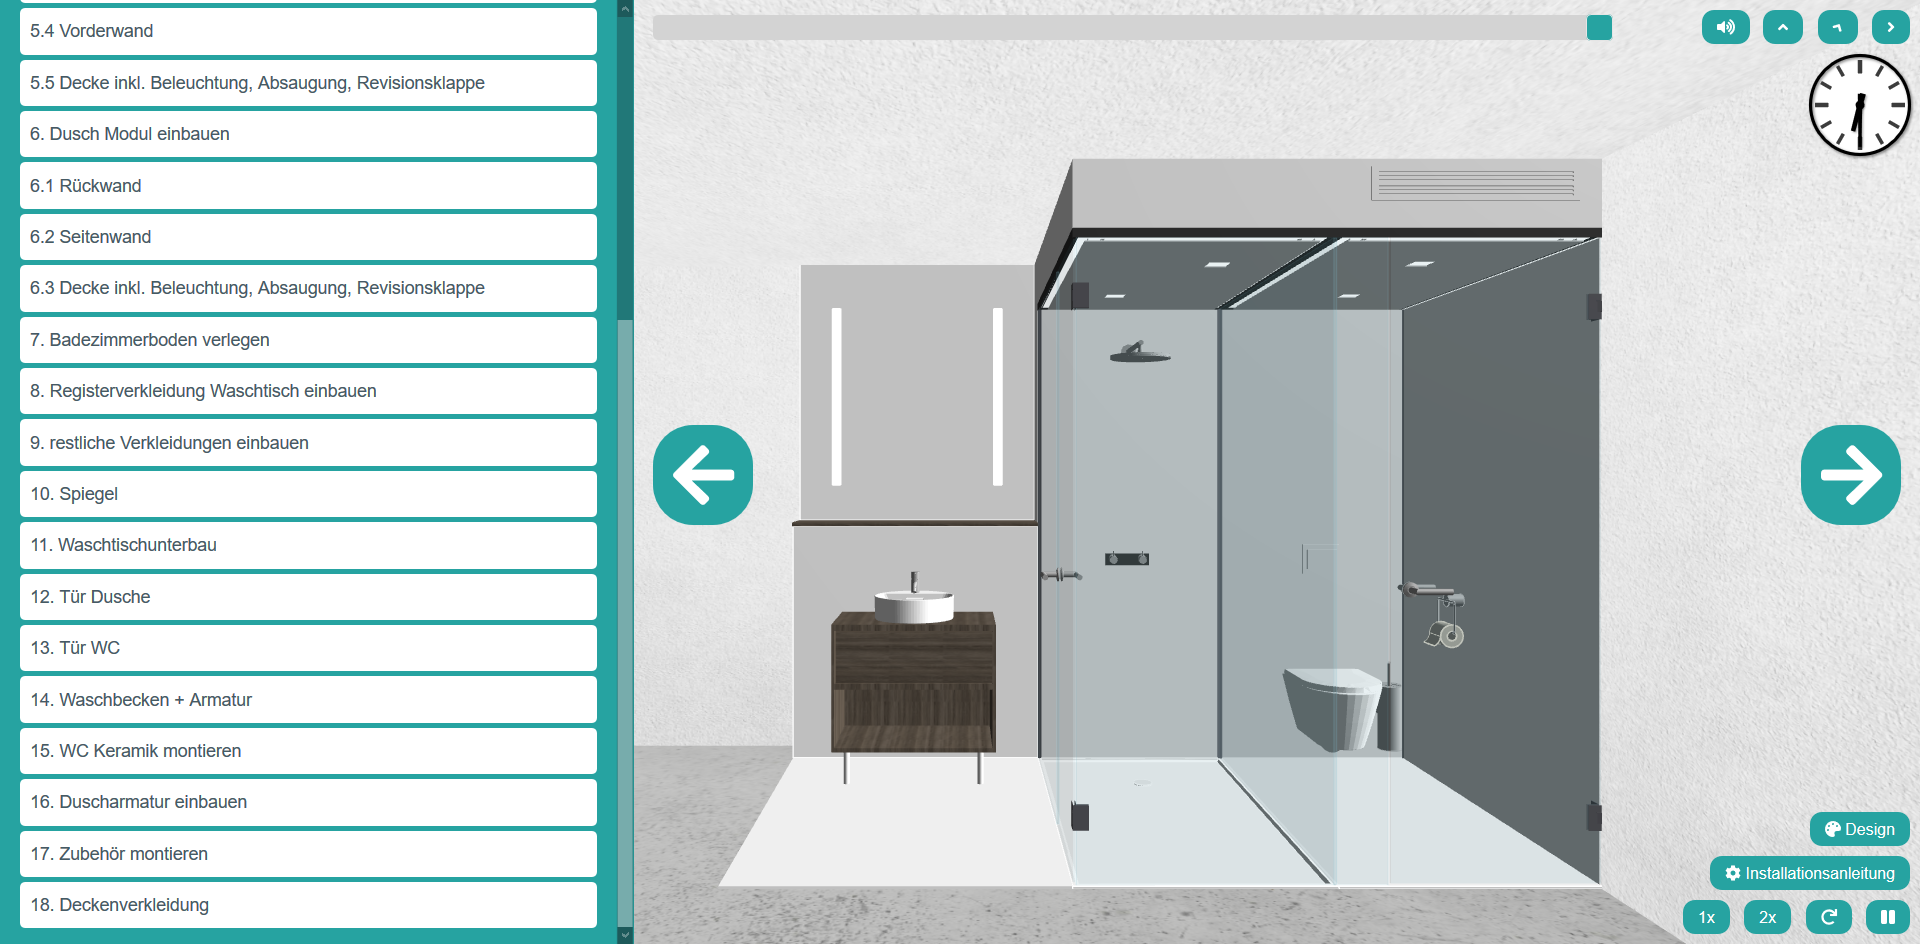
\includegraphics[width=0.65\linewidth]{images/Screenshot_front.png}
			\caption{Bad Designer; Frontalansicht}
\end{figure}

	
\begin{figure}[h]
    \centering
    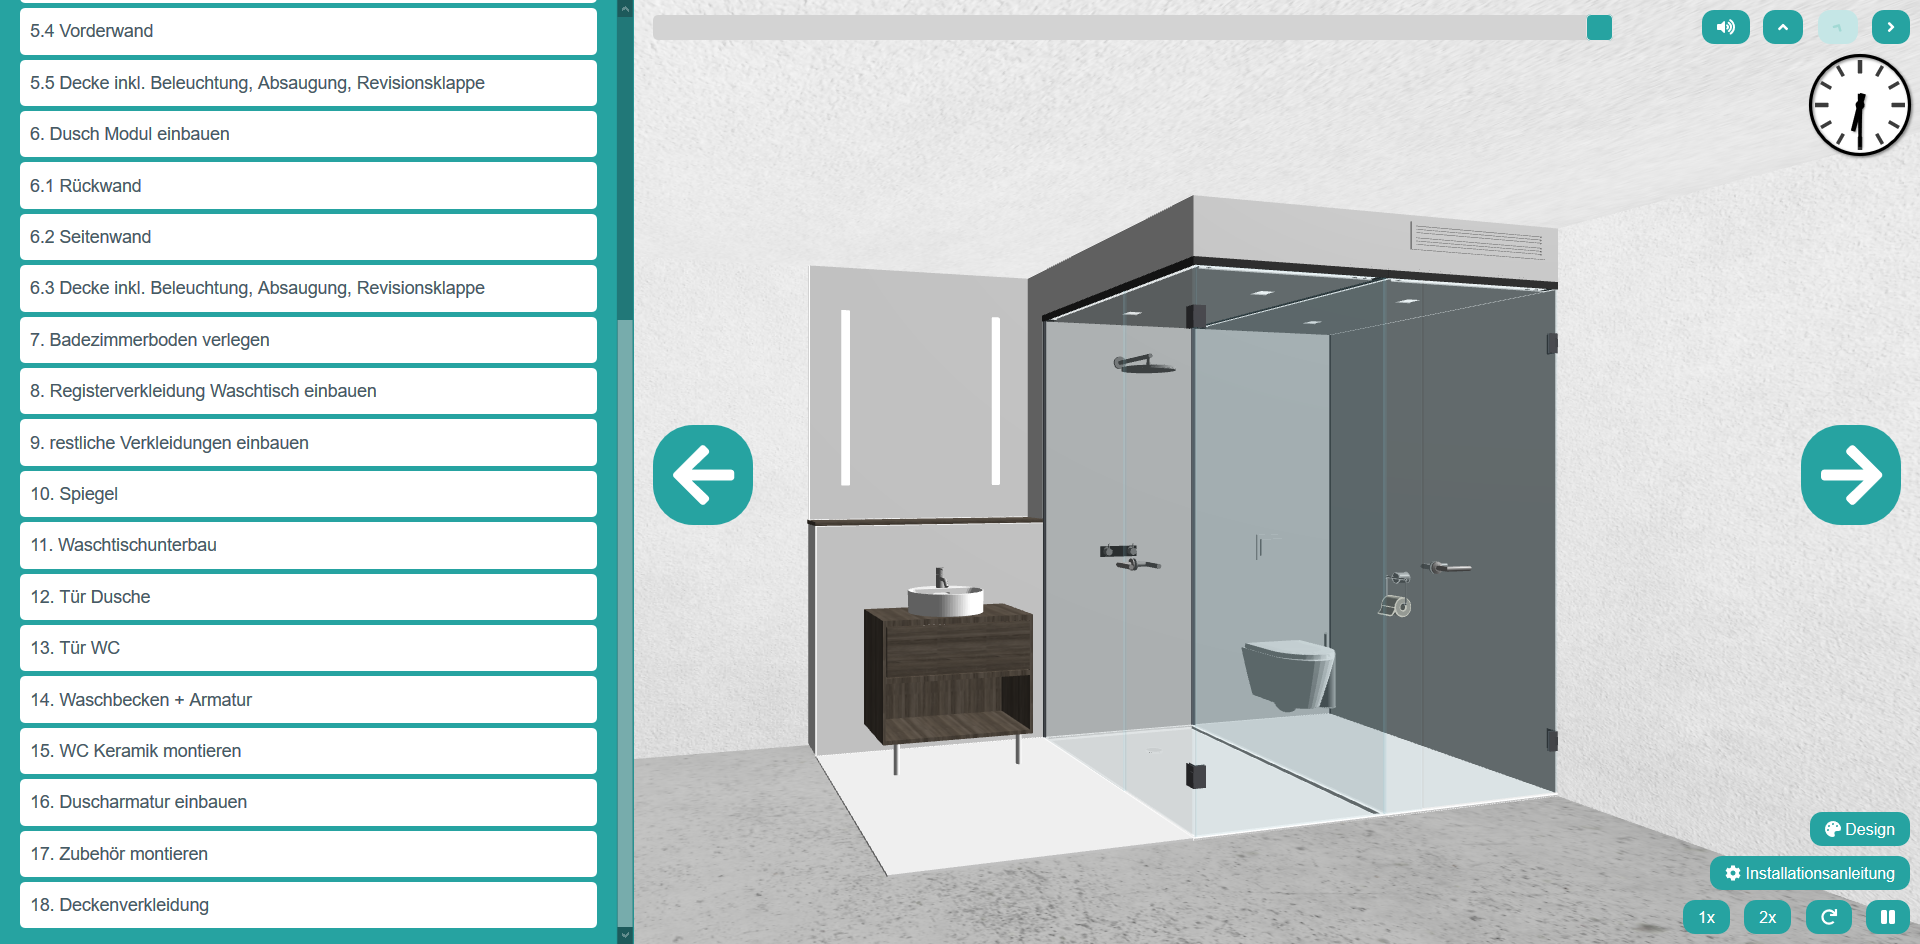
\includegraphics[width=0.65\linewidth]{images/Screenshot_schraeg.png}
	\caption{Bad Designer; Schrägansicht}
\end{figure}	


\begin{figure}[h]
    \centering
    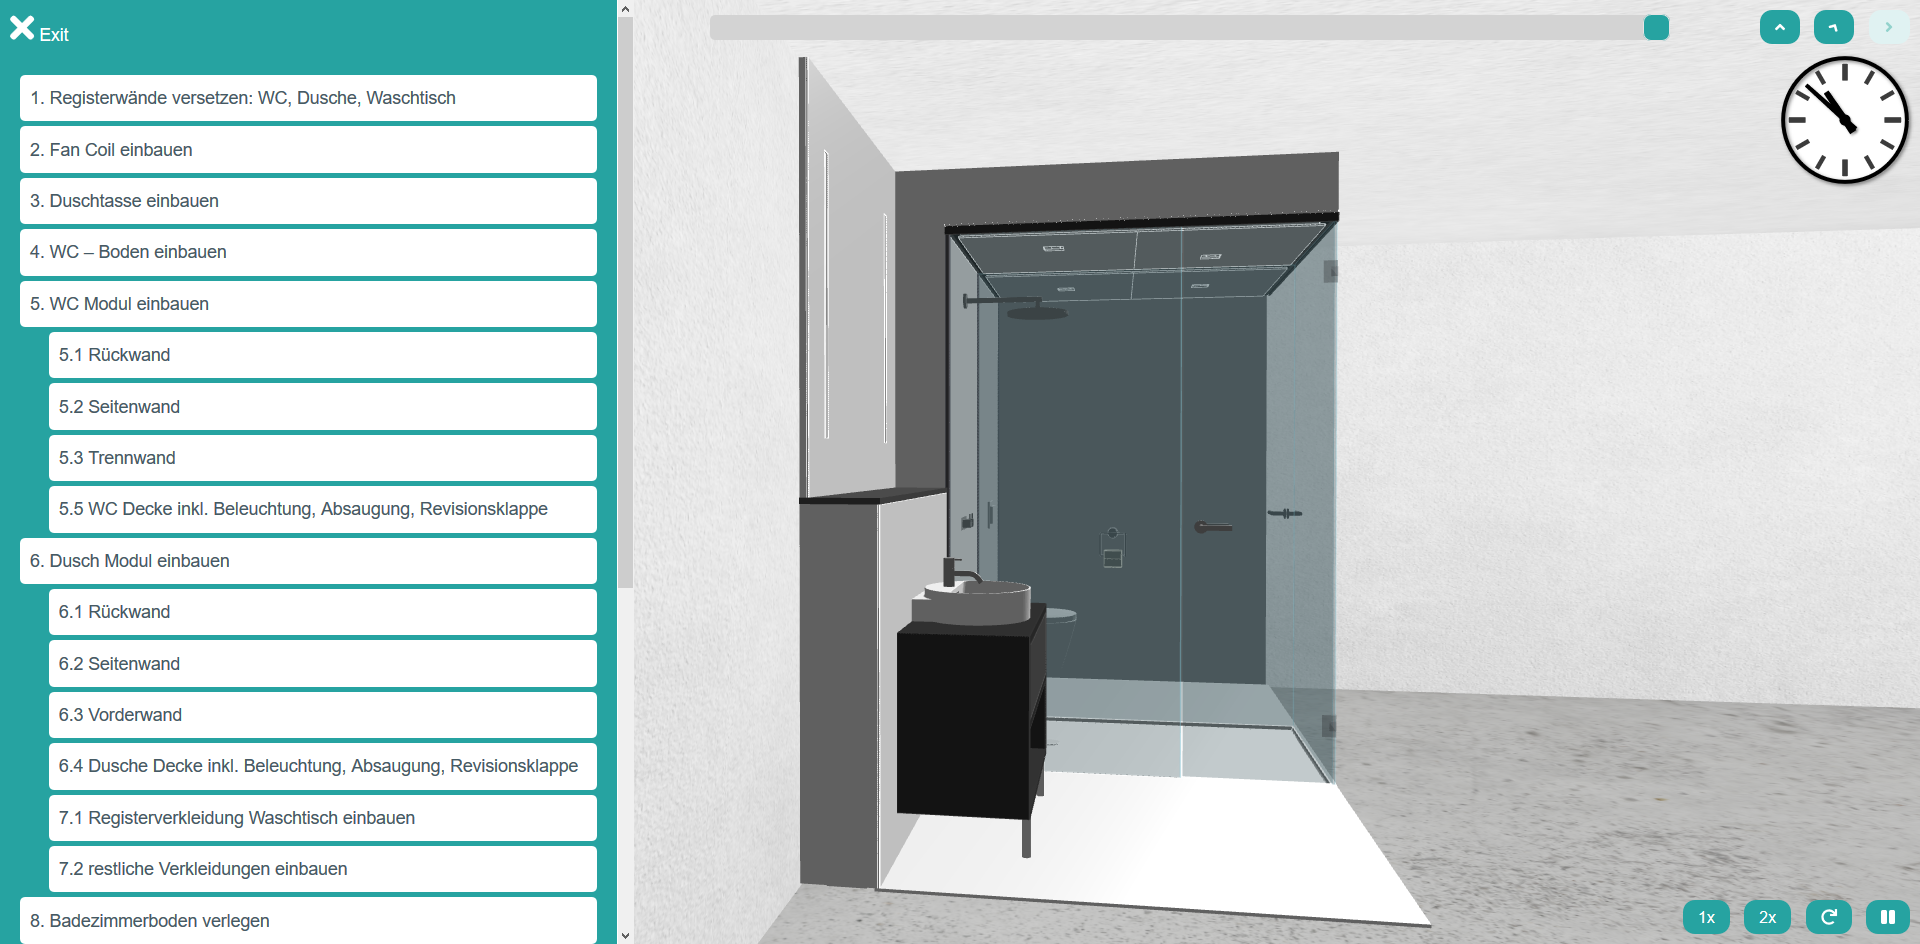
\includegraphics[width=0.65\linewidth]{images/Screenshot_seite.png}
	\caption{Bad Designer; Seitenansicht}
\end{figure}

\end{abstract}

	\newpage
	\clearpage
\begin{otherlanguage}{english}
\begin{abstract}

% \begin{enumerate}
\begin{itemize}
	\item {\em Definition of the project} \\ In order to present the customers of {\projectpartner} a visualization of a custom-made modular bath it is necessary to have a precise and detailed illustration. This is especially important for the custom design, the components and for the construction manual. As the model will be showed to the assembler as well it is important that it is possible to build it with the manual the application provides. The progress and the complete bath can be viewed from multiple angles with the intention of making the concept clearer and simpler for all. As it is a web application it can be run on every operating system and thanks to Electron locally runable without an internet connection. Up to now this was done with presentation videos, but they were too inflexible and time-consuming. Moreover, the bath was only visible from one angle, the model was not interactive and customer requirements could not be implemented immediately. The tool is as intuitive as possible and does not require special resources.
	
	\item {\em Implementation} \\ The web-app is based on the commonly used technologies HTML, JavaScript, Three.js and WebGL. This allows it to be run on every operating system and any modern browser. It only requires a internet connection. The mentioned technologies were uses because they are all robust, future-proof, well documented and extendable. Thanks to these attributes they are perfect fit for the application and make it easier to service.
	
	\item {\em Results} \\ The software was delivered after the thesis to the company {\projectpartner}. Demonstrations and tutorials were provided to the future users by the developing team. The work is publicly accessible on this website \url{http://vm85.htl-leonding.ac.at/}.
\end{itemize}

\clearpage \newpage

\begin{figure}[h]
    \centering
    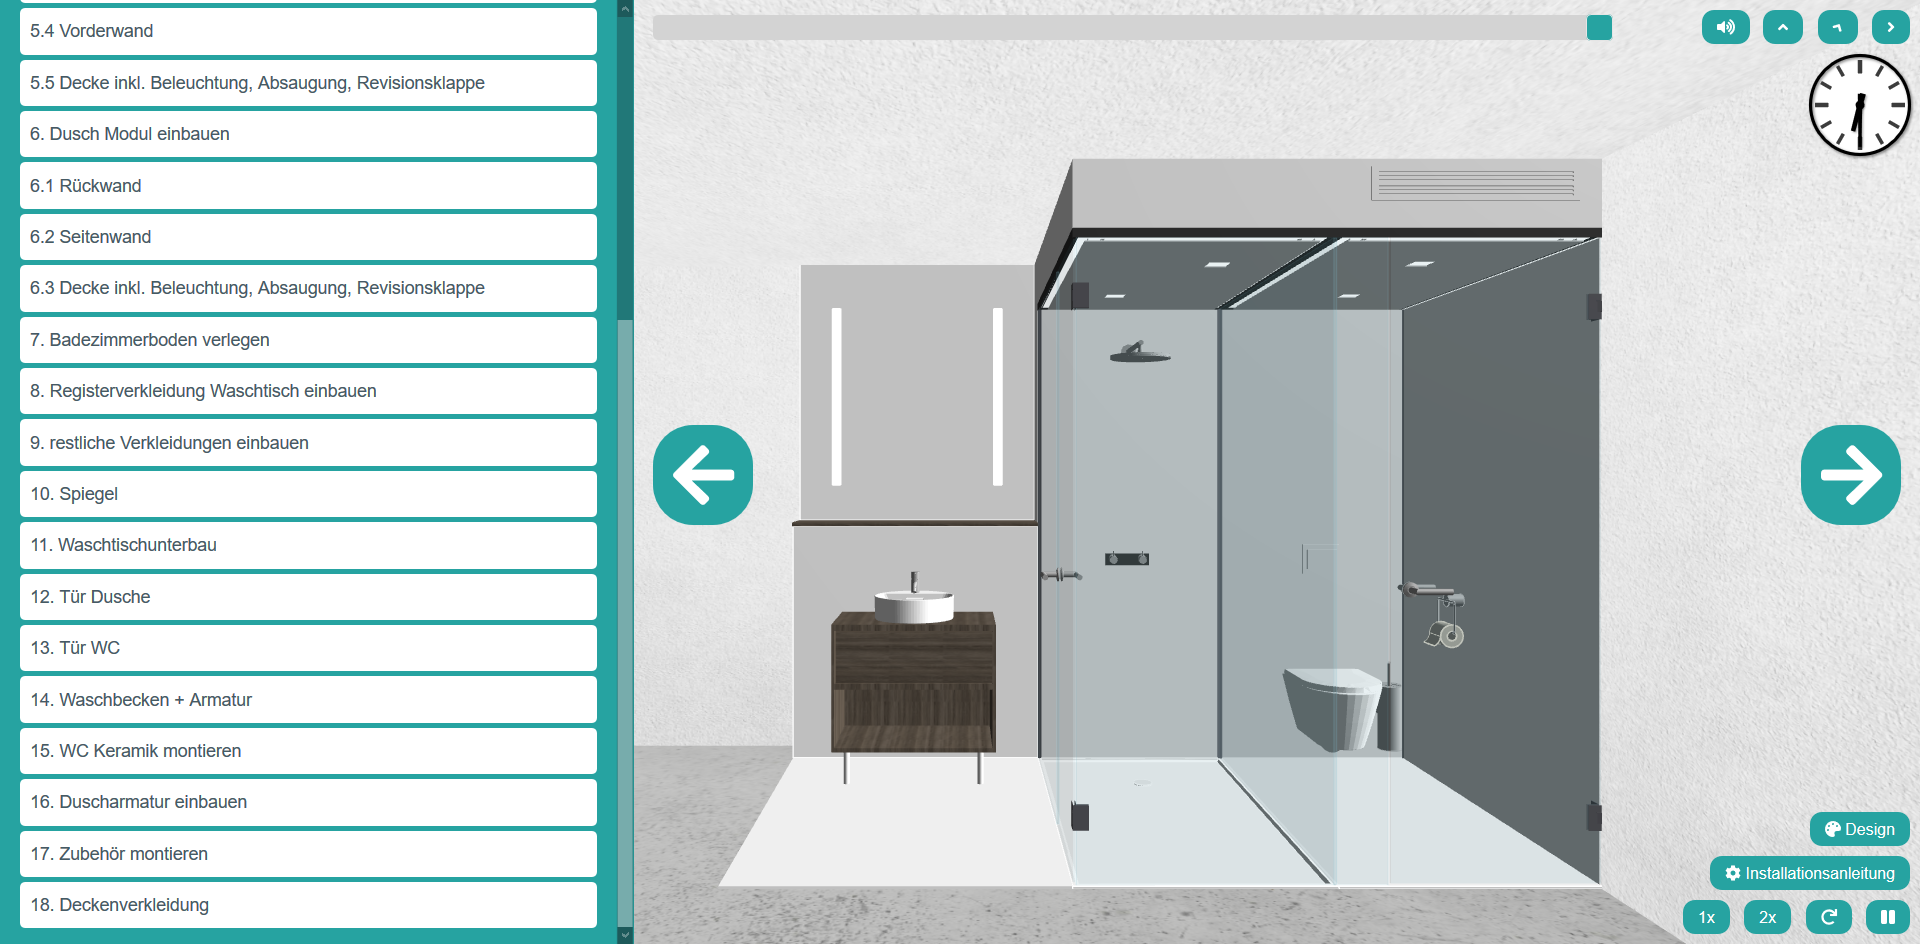
\includegraphics[width=0.65\textwidth]{images/Screenshot_front.png}
		\caption{Bad Designer; Frontal view}
\end{figure}



\begin{figure}[h]
    \centering
    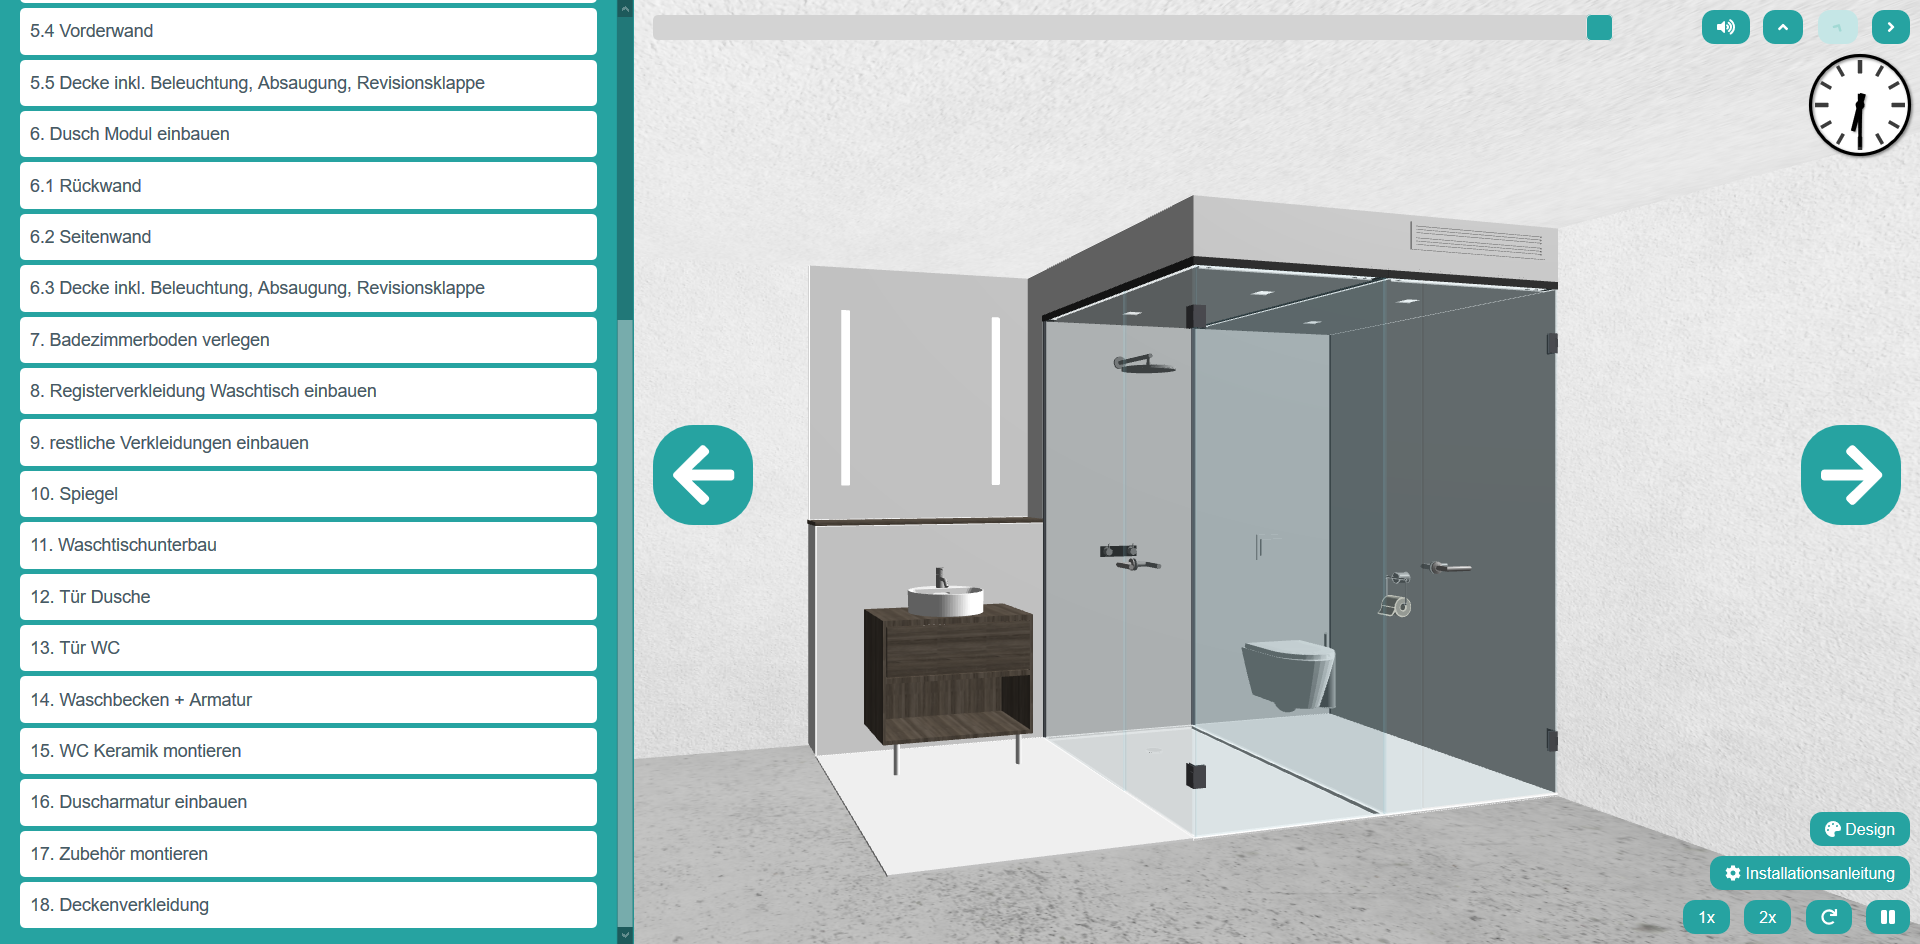
\includegraphics[width=0.65\textwidth]{images/Screenshot_schraeg.png}
		\caption{Bad Designer; Oblique view }
\end{figure}


\begin{figure}[h]
    \centering
    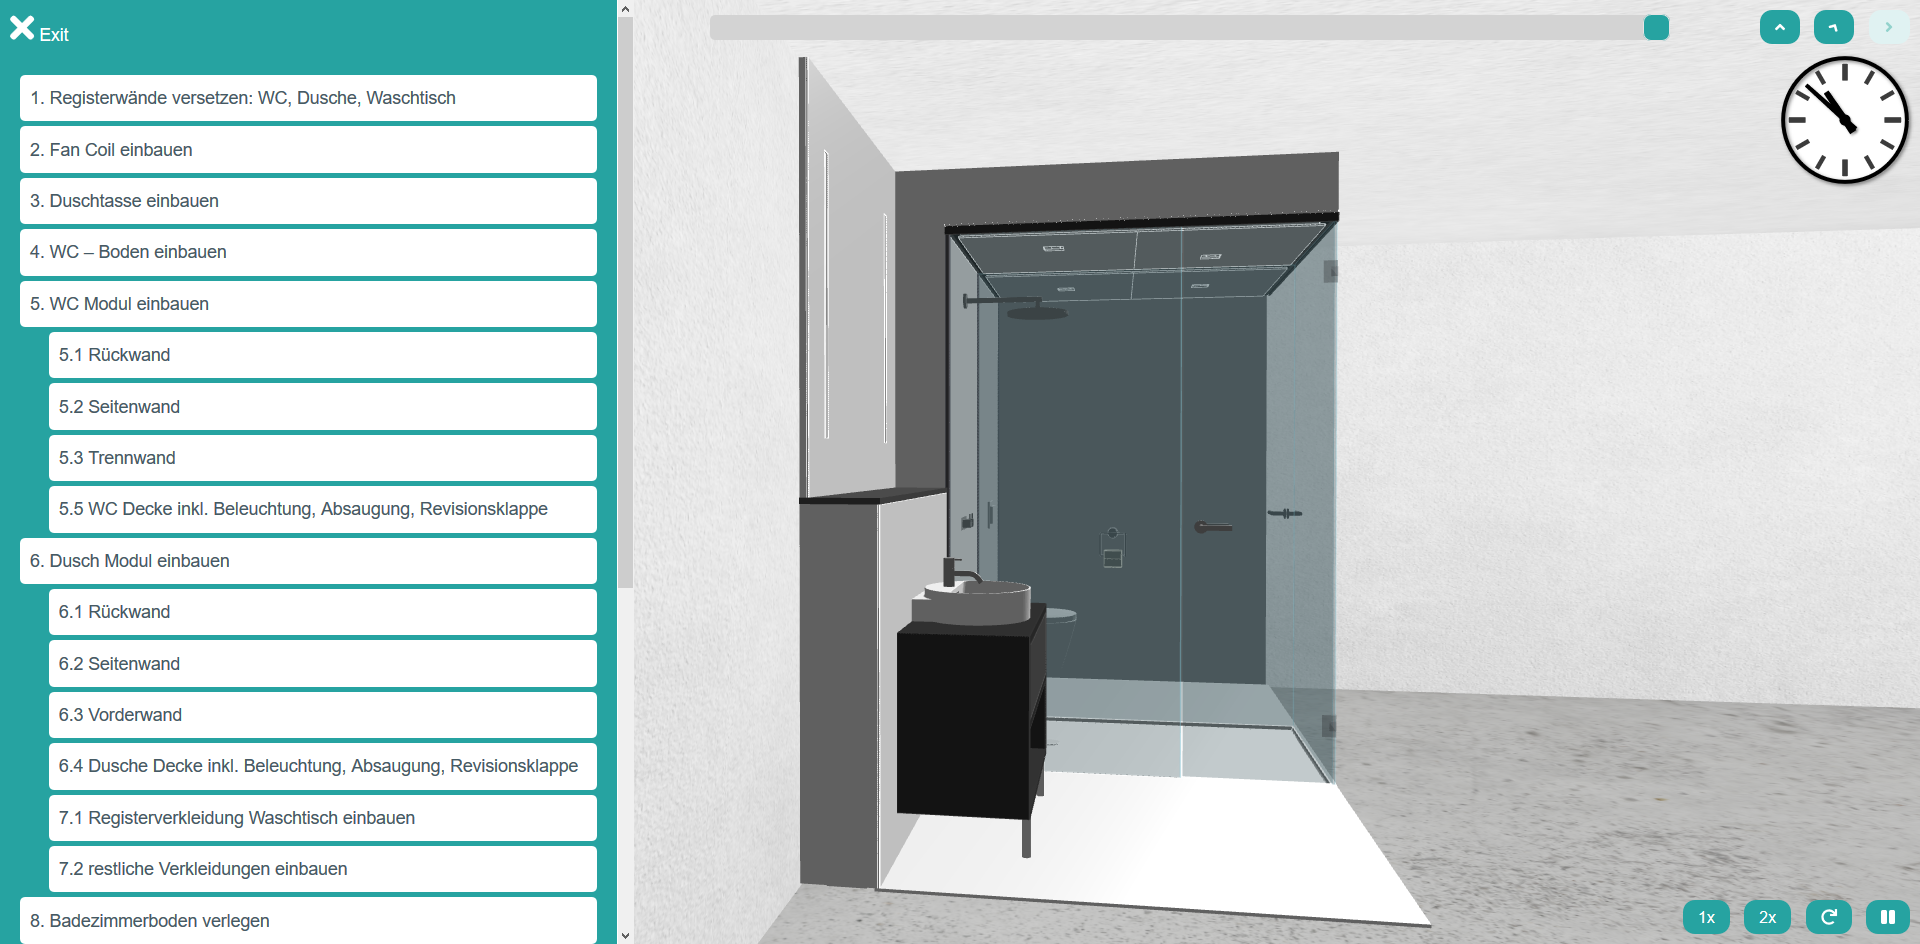
\includegraphics[width=0.65\textwidth]{images/Screenshot_seite.png}
		\caption{Bad Designer; Side view}
\end{figure}

\end{abstract}
\end{otherlanguage}

\newpage
\clearpage
\section*{Danksagungen}
Wir möchten uns sehr herzlich bei unserem Diplomarbeitsbetreuer {\supervisor} bedanken der uns stets fachlich und persönlich unterstützt hat und immer an unserer Seite stand. Einen großen Dank möchten wir auch an unseren Auftraggeber die {\projectpartner} richten die uns das Vertrauen geschenkt hat. Für das Vermitteln der Diplomarbeit möchten wir uns bei Prof. Dipl.-Ing. Richard Kainerstorfer bedanken.
\\ \\
Ein großer Dank gilt auch unseren Familien und Freunden die in der Zeit der Erstellung dieser Arbeit für uns da waren und uns unterstützt haben. % Declaration of Academic Honesty, Abstracts, Acknowledgments, 
\section*{Auftraggeber}

{\projectpartner} ist ein Unternehmen mit Sitz in Leonding, das sich auf Innenarchitektur und Glasdekore spezialisiert hat, 
die verschiedenste Räumlichkeiten wie Bars, Hotelzimmer und etc. für den Kunden attraktiver machen. 
SanMod-Bäder bieten individuelle, freistehende Sanitärmodule für einen flexiblen und zeitsparenden Einbau in Gebäuden
Die Anordnung der Module ist flexibel und richtet sich sowohl nach den räumlichen Vorgaben als auch nach der gewünschten 
Offenheit des Badezimmers zum restlichen Raum hin.
Auf dieser Basiskonstruktion werden sämtliche Bestandteile eines hochwertigen Hotel-Badezimmers montiert.



\includegraphics[scale=.3,right]{images/LL_Logo_skaliert.png} % Auftraggeber Info 


\tableofcontents

\chapter{Einleitung}
\section{Ausgangslage}
{\projectpartner} ist ein Unternehmen mit Sitz in Leonding, das sich auf Innenarchitektur und Glasdekore spezialisiert hat, die verschiedenste Räumlichkeiten wie Bars, Hotelzimmer und etc. für den Kunden attraktiver machen. SanMod-Bäder bieten individuelle, freistehende Sanitärmodule für einen flexiblen und zeitsparenden Einbau in Gebäuden. Zurzeit werden die Bäder dem Kunden mit einem Video präsentiert. Diese Methode bringt aber Nachteile mit sich da die Bäder immer nur aus einer Perspektive gezeigt werden, die Modelle unflexibel sind, nicht interaktiv und Kundenwünsche nicht sofort umgesetzt werden können. Diese Probleme werden durch die Applikation behoben und macht es möglich die Designentwürfe für spätere Zwecke abzuspeichern.

\section{Zielsetzung}
Das Ziel ist es die Planung zu erleichtern und gegebenenfalls Änderungen sofort im Kundengespräch umzusetzen. Durch diese virtuelle Stütze können sich alle Beteiligten das fertige Bad besser vorstellen, und mögliche Missverständnisse sofort klären. Kundengespräche werden dadurch aufgewertet und effizienter.

\section{Aufbau der Diplomarbeit}
Die Diplomarbeit ist in drei Teile gegliedert. 
Der erste Teil besteht aus den verwendeten Technologien.
Der zweite Teil geht näher auf die Grundlagen und Methoden der Arbeit ein.
Der dritte und letzte Teil behandelt die Umsetzung und Realisierung des Projektes.
Außerdem wird hier auf die Systemarchitektur eingegangen und die Implementierung so wie
der Release der Diplomarbeit.


\begin{figure}
\begin{center}
	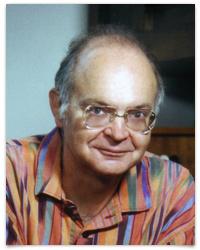
\includegraphics[scale=.5]{images/don_knuth.jpg}
\end{center}
	\caption{Don Knuth, the inventor of \TeX}
	\label{fig:sample}
\end{figure}

\section{Basic Terminology}
As usual the very basic terminology is briefly explained here. Most probably the explanations here only scratch a surface level. More detailed explanations of terminology goes into chapter%~\ref{cha:theoretical-background}.

\section{Related Work and Projects}
Here a survey of other work in and around the area of the thesis is given. The reader shall see that the authors of the thesis know their field well and understand the developments there. Furthermore here is a good place to show what relevance the thesis in its field has.

\section{Structure of the Thesis}
%dsflkjas flaksjfl asdfj as lfjldsajflaksdjf sa dfjlasdkfj sadlfjasdklf als dfj l dfsdfsdfn chapter~\ref{cha:used-technologies} (\nameref{cha:used-technologies}) on page~\pageref{cha:used-technologies} we describe the used technologies.
Finally the reader is given a brief description what (s)he can expect in the thesis. Each chapter is introduced with a paragraph roughly describing its content.
\part{Verwendete Technologien}\label{part:Verwendete Technologien}
\chapter{Software}


\section{HTML5}

\section*{Erläuterung}
HTML5 ist die fünfte Generation der Hypertext Markup Language. HTML wird hauptsächlich zur Darstellung von Websites im Internet genutzt. Die HTML-Dateien werden dabei von einem Browser abgerufen und dargestellt.

\section*{Funktionalität}
Dadurch das HTML mit CSS und JavaScript um ein Design und Funktionen erweitert werden kann ist es sehr flexibel und vielseitig einsetzbar. Ganze Programme werden heute als WebApp programmiert und bieten denselben Funktionsumfang wie normale desktopbasierte Programme. Weil nur ein Browser benötigt wird um die Websites darzustellen sind sie außerdem plattformunabhängig.  


\section*{Verwendung}
HTML bildet das Fundament für den Bad-Designer, auf dem alle anderen Features aufbauen. Die Modelle der sanitären Anlagen werden hier geladen. Die restlichen Funktionen werden mit JavaScript implementiert.

\newpage
\clearpage

\section{JavaScript}

\section*{Erläuterung}
JavaScript ist eine Skriptsprache, die dazu dient, um HTML zu erweitern. Damit kann man auf Benutzerinteraktionen reagieren und auswerten, Inhalte verändern, generieren und nachladen. Somit sind die Seiten dynamisch und ergänzen HTML und CSS so dass sie interaktiv werden. Des Weiteren wird JavaScript auch für Server und Microcontroller verwendet. Eine bekannte serverseitige Plattform, nämlich Node.js, basiert auf der JavaScript-Laufzeitumgebung. 
\\
Die Syntax der 1995 erschienenen Sprache ähnelt der von C. Obwohl Java auf Gemeinsamkeiten vermuten lässt ist JavaScript deutlich anders und vieles abweichend implementiert. Durch die Variabilität ist es möglich objektorientiert, prozedural oder funktional zu programmieren.

\section*{Funktionalität}
JavaScript bildet mit seinen umfangreichen Funktionen ein Grundgerüst für die meisten Dinge. Animationen, Berechnungen, Benutzer Interaktionen und Datenverarbeitung werden es dadurch möglich.


\section*{Verwendung}
Das Laden der Modelle, Animationen, Benutzer Eingaben und Berechnungen wurden allesamt in JavaScript realisiert. JavaScript ist der wichtigste Bestandteil der Arbeit, die meisten Funktionen wären ohne diese Skriptsprache nicht möglich.  Außerdem basiert die Bibliothek three.js auf dieser Sprache und erweitert sie. Mehr zu three.js wird auf den folgenden Seiten näher erläutert.


\newpage
\clearpage


\section{WebGL}

\section*{Erläuterung}
WebGL, kurz für Web Graphics Library, ist eine auf JavaScript basierende Programmierschnittstelle, die es ermöglicht 3D-Grafiken hardwarebeschleunigt im Webbrowser ohne zusätzliche Erweiterungen, Bibliotheken und Technologien darzustellen. Des Weiteren basiert WebGL auf den Spezifikationen von OpenGL ES, kurz für Open Graphics Library for Embedded Systems. Diese beschreibt eine plattform- und sprachenunabhängige Programmierschnittstelle für die Entwicklung von 3D-Computergrafiken. 
\\
Die 2011 erschienene Library ist lizenzfrei von der Khronos Group und Mozilla entwickelt worden. Mit der Zeit haben immer mehr Unternehmen die Entwicklung unterstützt, dazu zählen unteranderem Google Chrome, AMD, Ericsson, Nvidia und Opera. 


\section*{Funktionalität}
Dadurch das die Grafik-Bibliothek im Browser läuft, ist sie plattformunabhängig und hat unteranderem deshalb auch eine große Reichweite. Zusätzlich gestattet sie Grafikern mit den beliebten Softwarewerkzeugen wie Blender, Maya oder CopperCube zu arbeiten ohne sich um die Darstellung anschließend kümmern zu müssen. WebGL konfiguriert und verarbeitet die Modelle für den Browser.

\section*{Verwendung}
WebGL kann für eine Vielzahl von Dingen verwendet werden, durch immer leistungsfähigere Geräte und Anwendungen wird das Anwendungsgebiet größer. Hauptsächlich wird es für 3D Modelle im Internet genutzt. Vor allem im Marketing Bereich wird die Anwendung kontinuierlich beliebter, da die Hersteller nun die Möglichkeit haben dem Kunden das Produkt auf einem zwei dimensionalen Bildschirm drei dimensional darzustellen. Dadurch steigt die Verkaufswahrscheinlichkeit wesentlich an da der Kunde eine Übersicht bekommt als hätte er sich das Produkt in echt angesehen.
\\
Das Laden der Badezimmer-Module übernimmt WebGL und dient gleichzeitig als Basis für three.js. Die ganzen Animationen und Effekte werden von dieser Bibliothek abgewickelt.



\newpage
\clearpage  

\section{NGINX}\label{sec:NGINX}
\section*{Erläuterung} 
NGINX ist eine modular aufgebaute Webserver-Software, die von Igor Sysoev entwickelt wurde. Sie wird unter der BSD-Lizenz[\ref{sec:BSD}] entwickelt. Die Software ist das erste Mal Ende 2004 erschienen und wird bis heute in regelmäßigen Abständen aktualisiert und weiterentwickelt. Außerdem wurde er in der weitverbreiteten und robusten Programmiersprache C geschrieben.

\section*{Funktionalität}
Der Webserver bietet durch den modularen Aufbau eine Vielzahl an möglichen Techniken, wie zum Beispiel Lastverteilung, Reverse proxying, SSL, Flash-Video-Streaming, WebSocket-Protokoll und vieles mehr. 


\section*{Verwendung}
NGINX gehört zu den marktführen und wird heutzutage bei rund
 42\% der 1.000 Webseiten ~\cite{nginxWorldWide} mit dem höchsten Traffic verwendet. 
 Als http-Server hat er in Österreich sogar knapp 10\% Marktanteil ~\cite{nginxAT}. 
\\
Der Webserver dient beim Bad-Designer als Back-End wo die ganzen Modelle vom Bad und die Website selbst gehostet werden.



\newpage
\clearpage

\section{AutoCAD}

\section*{Erläuterung}
AutoCAD ist ein von AutoDesk entwickelter grafischer Zeichungseditor. Dieser ermöglicht es speziell technische Zeichnungen zu modellieren. Außerdem ist es ein vektororientiertes Zeichentool, das auf den Grundlagen für komplizierte 3D-Objekte basiert wie Linien, Polylinien, Kreisen, Bögen und Texten.
\\
Durch die umfangreichen 3D-Funktionen findet das Programm primär in den Bereichen Maschinenbau, Architektur, Design, Geoinformatik häufig Verwendung. In den genannten Bereichen ist die Software konstitutiv und manche Bauwerke beziehungsweise Maschinen sind erst dadurch möglich gewesen.

\section*{Funktionalität}
Die von der Firma AutoDesk entwickelten Dateiformate .dwg sowie .dxf sind mittlerweile ein Industriestandard im Austausch von CAD-Daten. Dies ermöglicht es das die Dateien auf den verschiedensten Plattformen wie Windows, Unix und MacOS mit Hilfe des Editors verwendbar sind. Desweitern kann man es auch als WebApp und Mobile App für Smartphones und Tablets verwenden.

\section*{Verwendung}
Alle Module des Badezimmers sind in AutoCAD modelliert worden. Von den Registern bis hin zu den Modulen des Bades. Die sanitären Anlagen wurden von der Firma {\projectpartner} zur Verfügung gestellt.



\newpage

\begin{figure}
	\begin{center}
		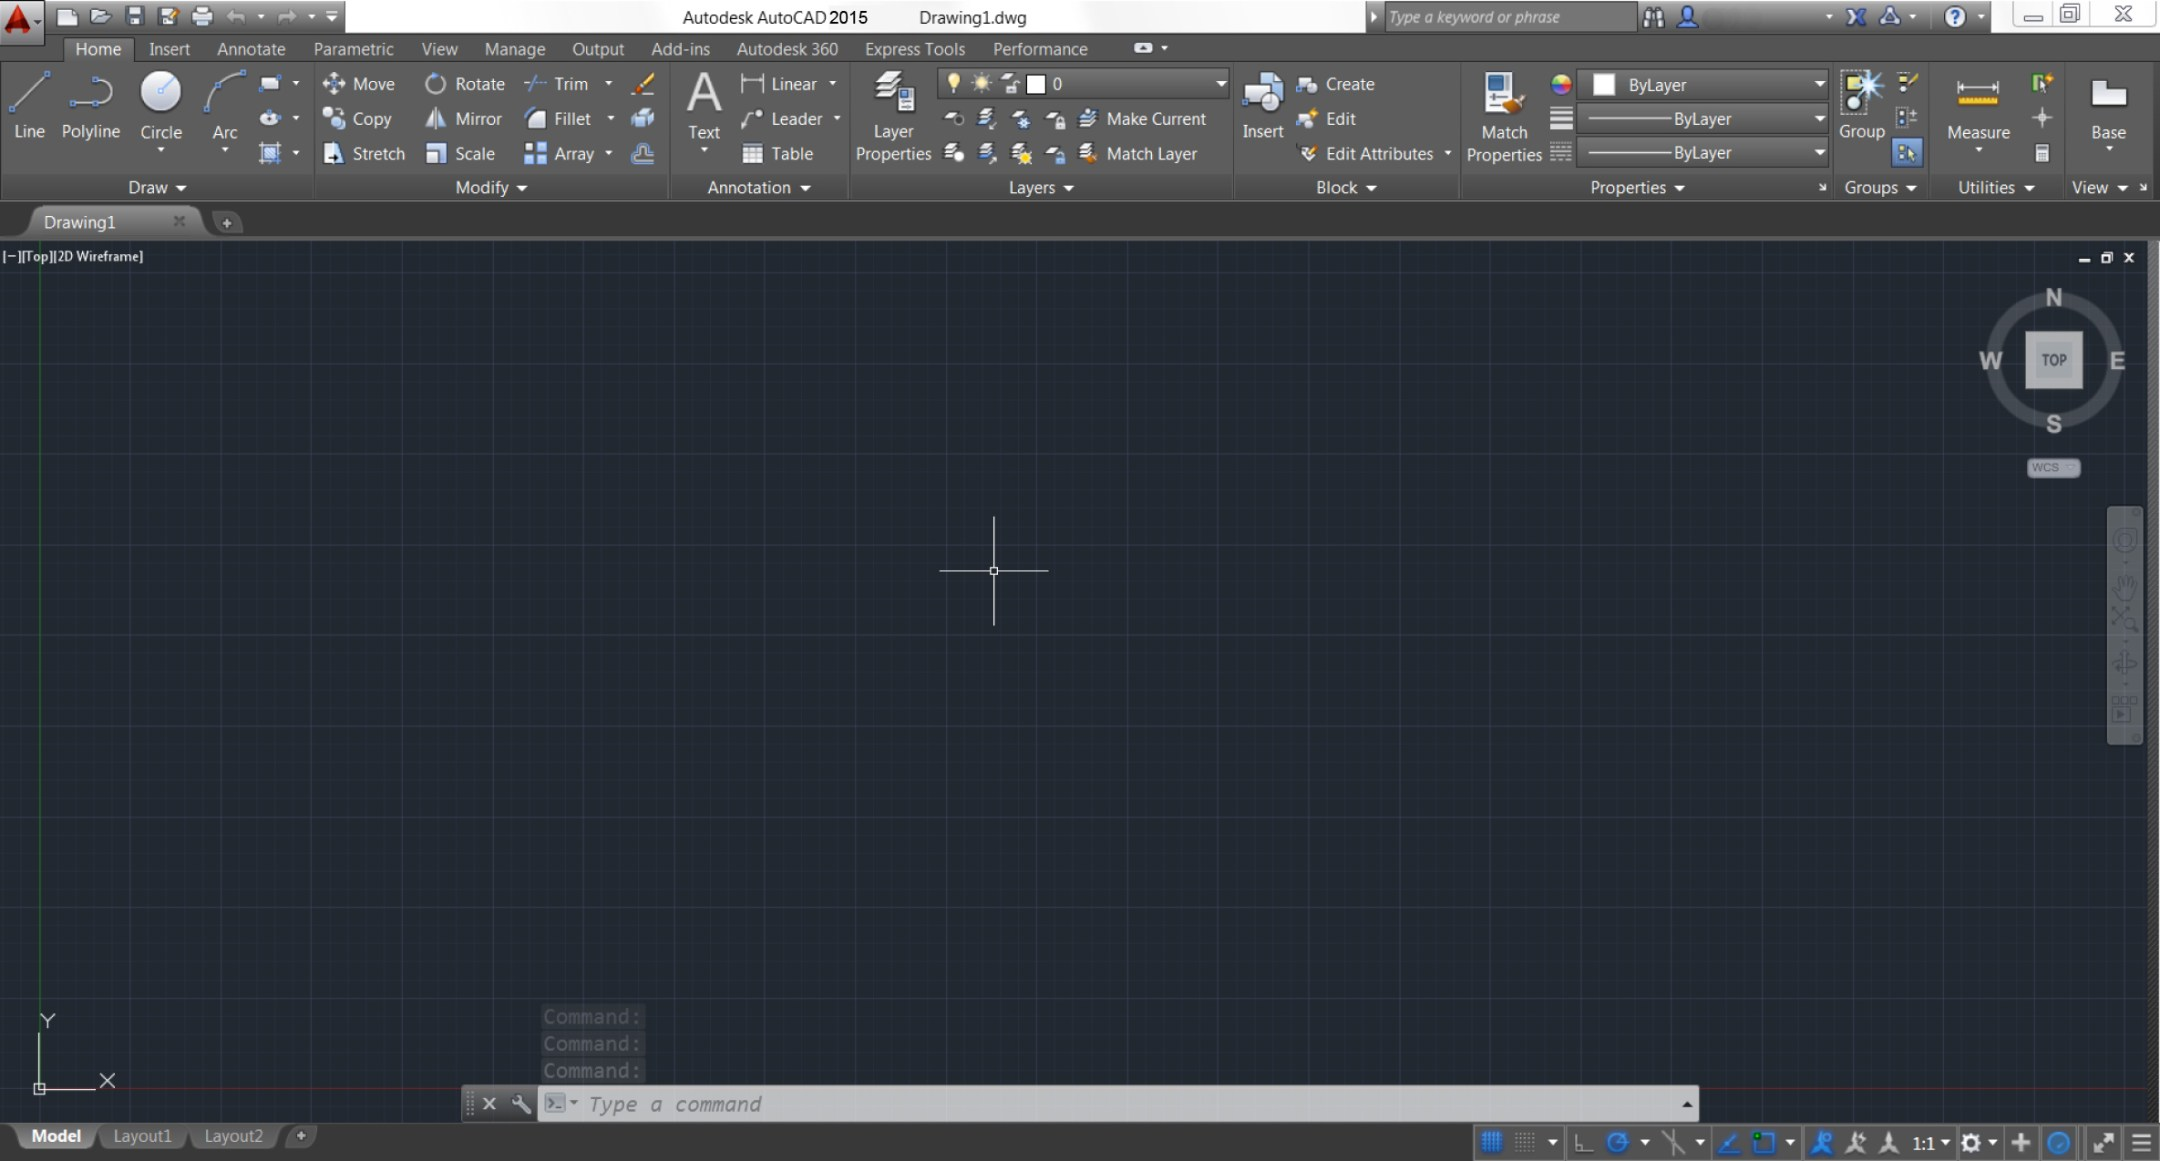
\includegraphics[width=16cm]{images/AutoCAD_UI.jpg}
		\caption{AutoCAD UI ~\cite{autocad}}
	\end{center}
\end{figure}


\newpage
\clearpage

\section{Electron}\label{sec:Electron}



\section*{Erläuterung}
Electron ist ein auf C++ und JavaScript basierendes quelloffenes Framework entwickelt von GitHub. Das 2013 erstmals erschienene Framework wird unter der MIT-Lizenz [\ref{sec:MIT}] vertrieben. Die auf Chromium und Node.js basierende Architektur ermöglicht es eine Cross-Platform-Desktop-Anwendung zu realisieren.

\section*{Funktionalität}
Webseiten die in HTML, CSS und JavaScript geschrieben wurden, können mit Electron in Desktop Anwendung umgewandelt werden ohne erheblichen Aufwand. Des Weiteren ist es möglich mit anderen Frameworks wie Vue.js und Angular zu arbeiten und anschließend zu einer Desktop App konvertieren. Das besondere daran ist, dass alle Electron-Executable auf den Betriebssystemen Windows, MacOS und Linux einwandfrei ohne Zutun ausführbar sind.


\section*{Verwendung}
Viele weitverbreitete und bekannte Programme wie die beliebten Editoren Atom und VS Code als auch die Messenger Discord und Skype wurden in Electron erstellt.
\\
Das Framework erlaubt es den Bad-Designer ohne eine Internetverbindung und lokal auf dem Rechner laufen zu lassen. Dafür muss nur das Executable heruntergeladen werden und schon ist es einsatzbereit.


\begin{figure}
	\begin{center}
		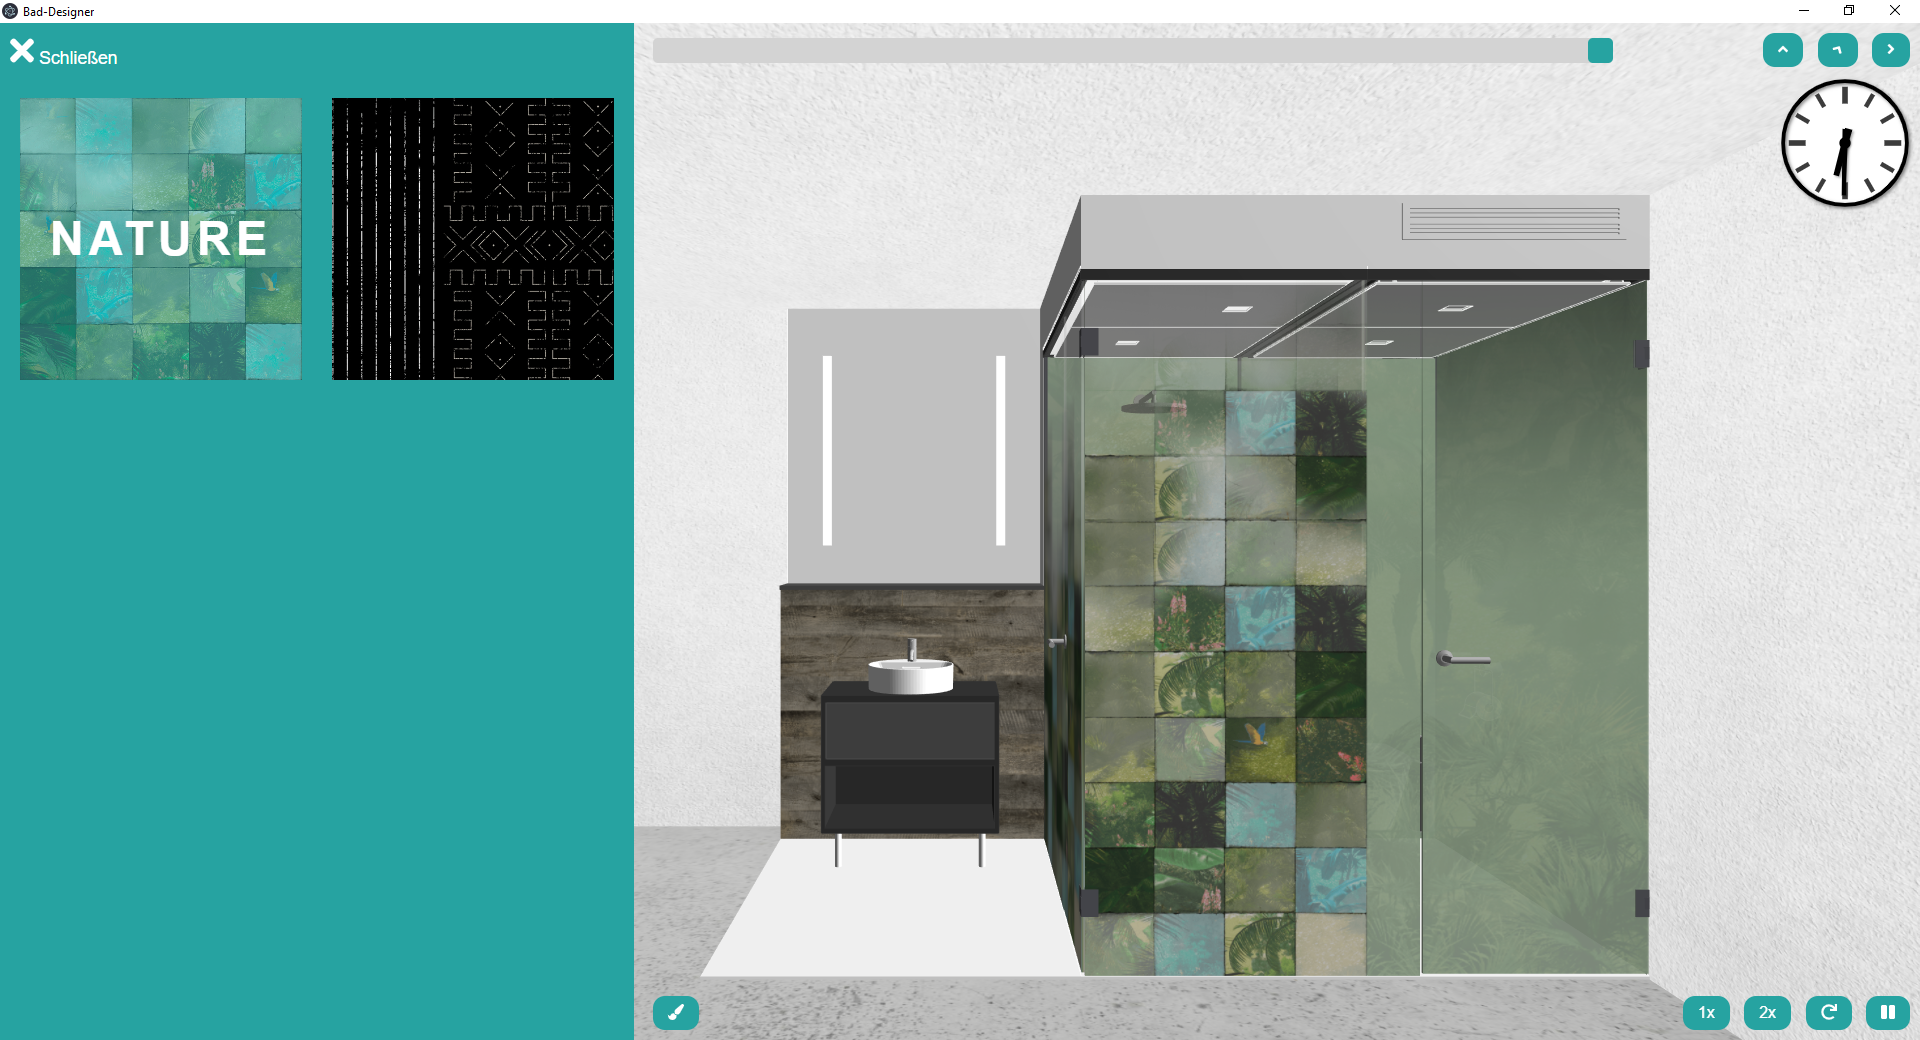
\includegraphics[width=16cm]{images/Electron_BD.png}
		\caption{Bad-Designer als Electron Anwendung}

	\end{center}
\end{figure}


\newpage
\clearpage
\section{Git}
\section*{Historie}
Git ist eine kostenlose Software, die für die verteilte Versionsverteilung von Dateien entwickelt wurde. Git wurde vom Linux-Kernel-Entwickler Linus Torvalds initiiert und entwickelt. Torvalds kam auf diese Idee da er zuvor BitKeeper nutzte, diese aber durch Lizenzänderungen kostenpflichtig wurde. 2005 begann er mit der Entwicklung des beliebten Versionsverwaltungsprogrammes. Dabei hatte er drei Anforderungen. Er wollte Unterstützung verteilter Arbeitsläufe, hohe Sicherheit gegen Verfälschung und hohe Effizienz. Mittlerweile ist der Maintainer Junio Hamano. 2018 wurde GitHub für 7,5 Milliarden US-Dollar von Microsoft übernommen. \\
Git läuft auf den Betriebssystemen Linux, MacOS und Windows. Das Programm selbst wurde in den Sprachen C, Perl, Tcl, Python und C++ geschrieben und unter der GNU-Lizenz [\ref{sec:GNU}] veröffentlicht. 
\\
Zu den Mitbewerbern von Git gehören GitLab und BitBucket. Laut der Plattform Open Hub, eine Website zur Katalogisierung von open-source-software, verwenden dort 71\% aller registrierten Projekte Git. \cite{GitMarketshare}
\\
Der Name stammt aus der britischen Umgangssprache der so viel wie Blödmann bedeutet. Torvalds wählte diesen Namen, weil er in der Softwarewelt unbenutzt war, kurz ist und er mit dem Namen einen Witz über sich selbst machte.
\\
\begin{quote}
	“I’m an egotistical bastard, and I name all my projects after myself. First ‘Linux’, now ‘Git’.” – \textbf{Linus Torvalds} \cite{TorvaldsJoke} 
\end{quote}
\clearpage
\newpage
\section*{Eigenschaften und Besonderheiten}
\subsection*{Branching}
Ein fester Bestandteil und Besonderheit an Git ist das Branching. Ein Branch ist dabei ein neuer Entwicklungszweig, dies ermöglicht es unabhängig vom Hauptzweig zu entwickeln und anschließend beide Zweige oder mehrere zu vereinen, dass sogenannte merging. Diese Verzweigungen sind in Git besonders effektiv implementiert, da sie lediglich eine Referenz auf einen bestimmten Commit sind.



\begin{figure}[!b]
	\begin{center}
		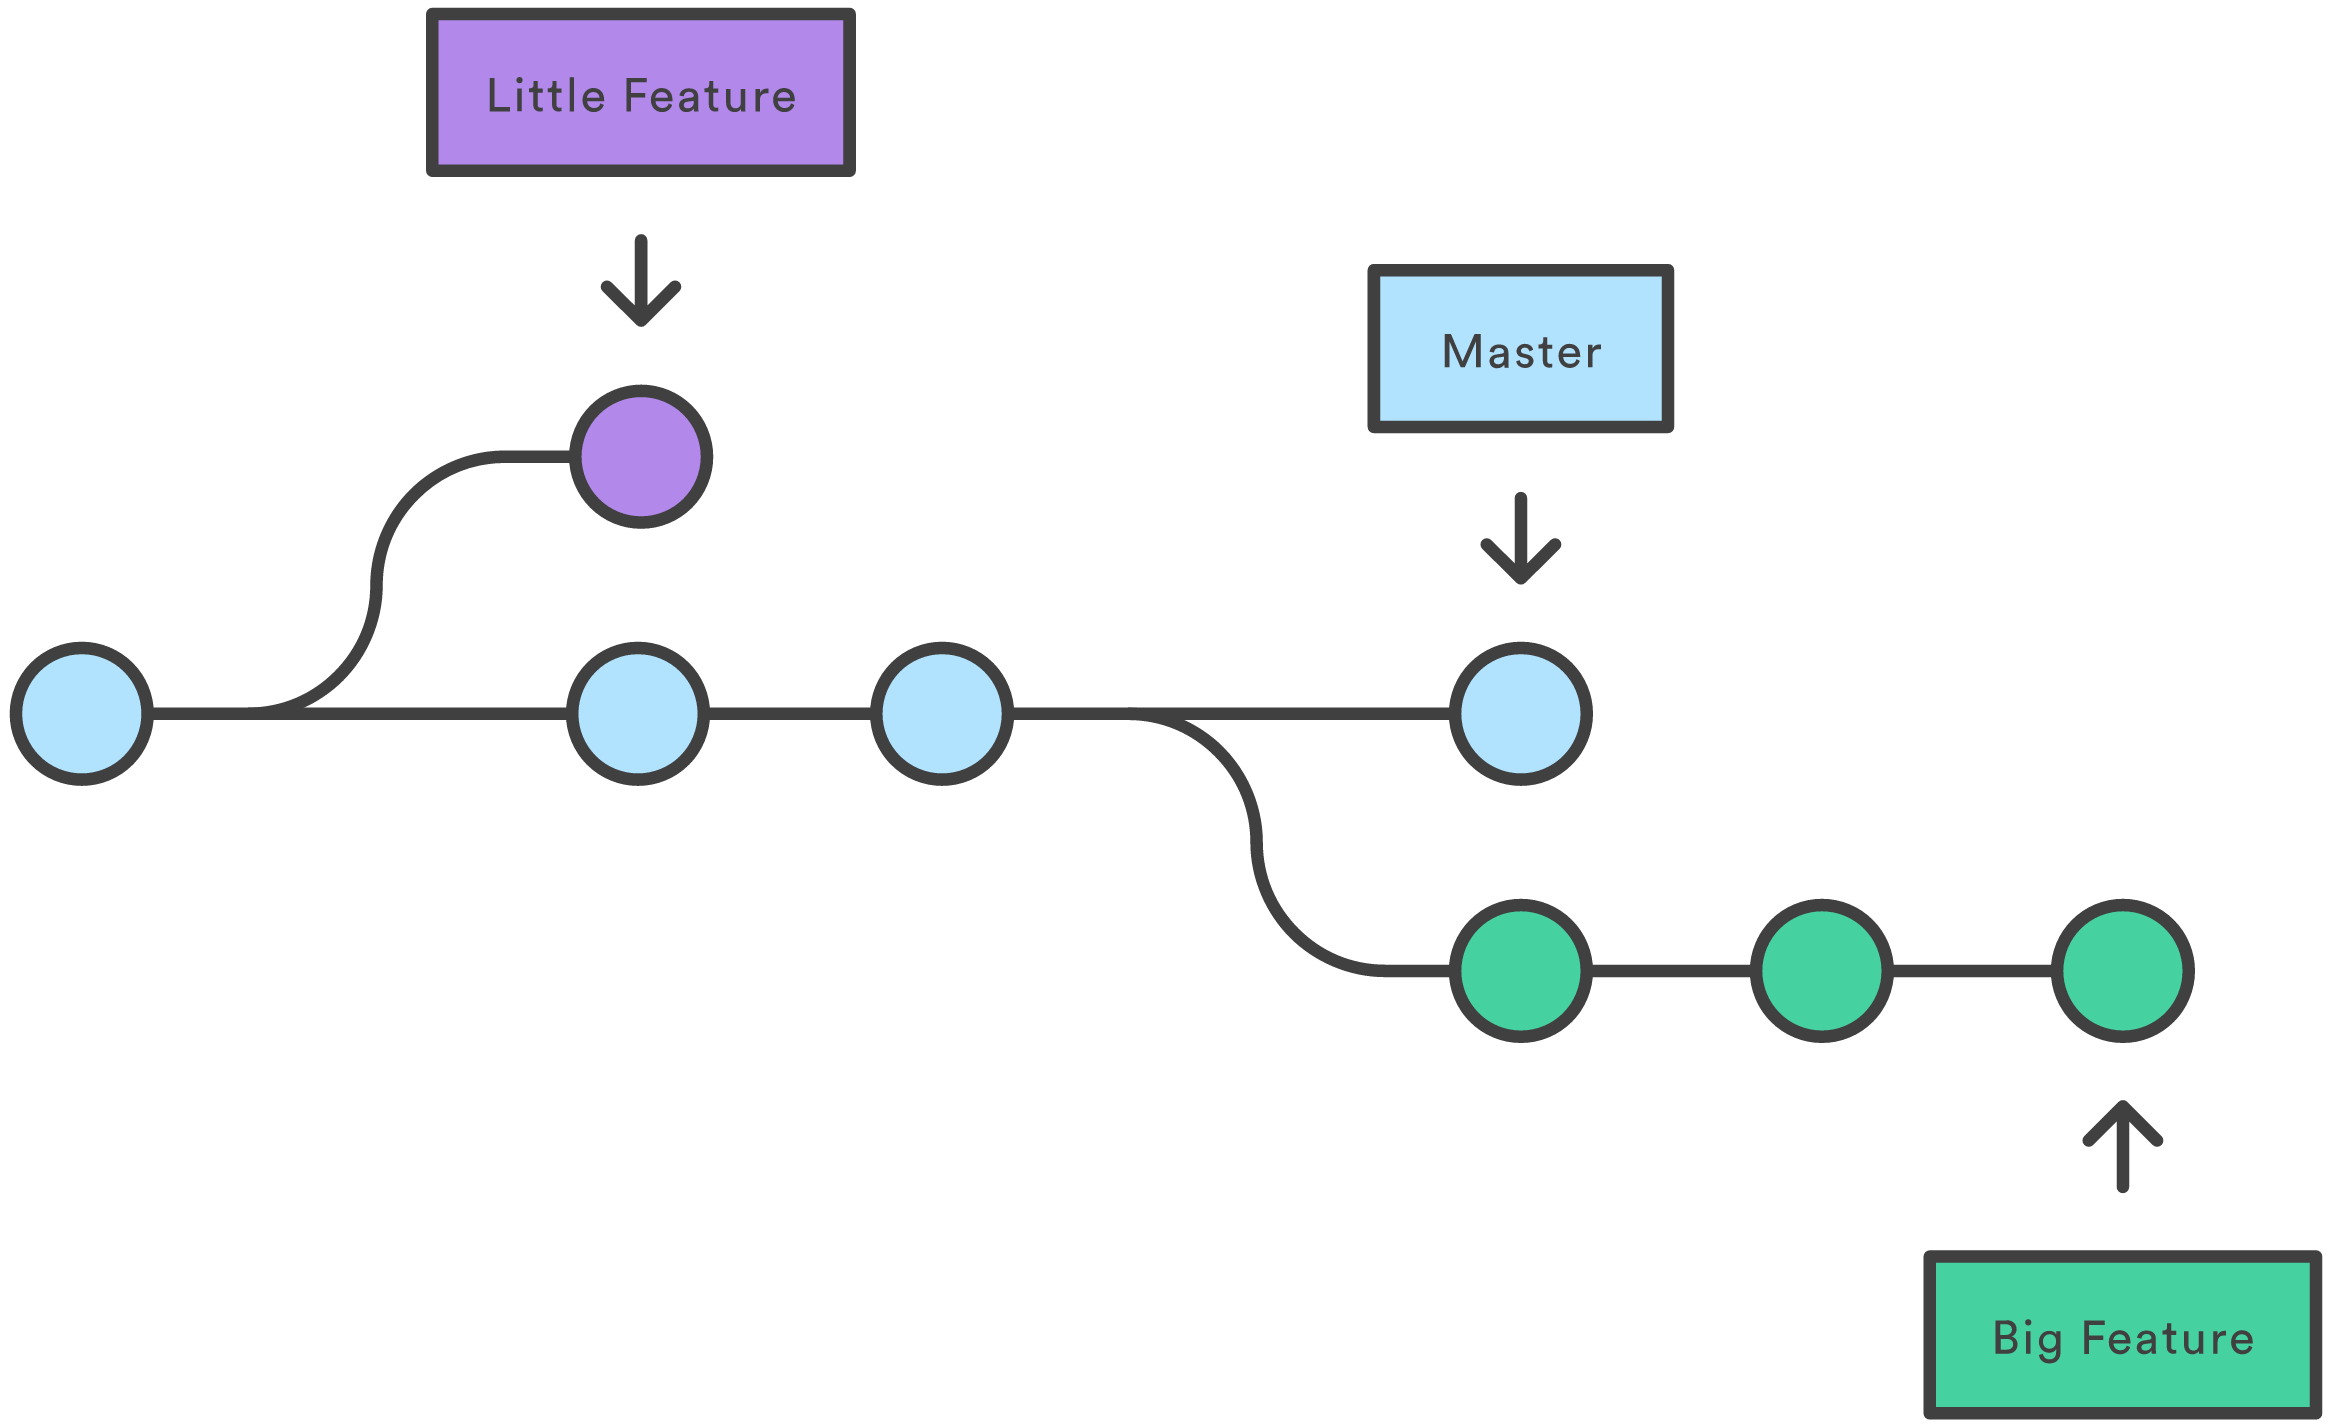
\includegraphics[width=16cm]{images/Git-Branches-1.png}
		\caption{Visualisierung von Zweigen in Git ~\cite{GitBranches}}
	\end{center}
\end{figure}
\newpage
\subsection*{Dezentralisierung}
Dadurch das jeder Benutzer sich eine lokale Kopie des Repositories samt Versionsgeschichte herunterladen kann, können die meisten Operationen ohne Internet durchgeführt werden. 

\subsection*{Sicherer Datentransfer}
Git bietet eine Vielzahl an unterschiedlichen Netzwerkprotokollen, um Daten zwischen Repositories zu übertragen. Das gängigste ist aber das sichere SSH Protokoll für Schreiboperationen und ein eigens entwickeltes Protokoll für das Fetchen und Clonen genutzt wird.

\subsection*{Sicherung der Projektgeschichte}
In Git ist es nicht möglich die Versionsgeschichte zu manipulieren. Das ist dem Hash-Wert geschuldet der bei jeder Revision (Commit) gespeichert wird. Dieser Wert basiert immer auf der vollständigen Geschichte, die bis zu jener Revision vorangegangen ist. 



\chapter{Dateien}

\section{.FBX}
~\cite{FBX_01} ~\cite{FBX_02}
\section*{Erläuterung}
3D-Objekte, 2d-Objekte mit Objekthöhe, Lichtquellen, Kameras und Materialien werden in dem vom AutoDesk entwickelten Dateiformat gespeichert. Das Universalformat, das bedeutet, dass es von diversen Programmen geöffnet werden kann, enthält unteranderem auch Übergänge, Video- und Audiodateien. 

\section*{Funktionalität}
Dadurch das FBX-Dateien die volle Funktionalität und Wiedergabetreue der Originaldatei beibehalten, ist es zum Beispiel möglich mit Cinema 4D, 3D Studio Max und PowerAnimator den Projektentwurf zu bearbeiten obwohl er davor in AutoCAD erstellt wurde. 

\section*{Verwendung}

\clearpage
\newpage

\section{.OBJ}
~\cite{OBJ_01}~\cite{OBJ_02}
\section*{Erläuterung}
Das offene Dateiformat .obj dient zum Speichern von dreidimensionalen geometrischen Formen. Das von Wavefront Technologies erstmals 1989 veröffentlichte Format gilt als universelles Dateiformat für Dreidimensionale-Grafikbearbeitungsprogramme. Daher eignet es sich für sowohl plattform- als auch programmübergreifende Weitergabe von Modellen.

\section*{Funktionalität}
Das OBJ-Format speichert lediglich die geometrischen Eigenschaften wie die Koordinaten der Ecken, Texturen, Normalen, Flächen und Glättungen. Die Oberflächenschattierungen können durch Referenzen auf .mtl-Dateien implementiert werden.

\section*{Verwendung}

\clearpage
\newpage

\section{.GLB}
~\cite{GLB_01}
\section*{Erläuterung}
In GLB-Dateien werden Repräsentationen von dreidimensionalen Modellen im GL Transmission Format, binär abgespeichert. Das GL Transmission Format speichert dreidimensionale Objekte im JSON-Format ab. Des Weiteren werden Kameras, Materialien, Animationen und Meshes binär in der GLB-Datei abgespeichert. 
\section*{Funktionalität}
Durch die kompakten Dateigrößen und das JSON-Format können so komplette dreidimensionale Szenen Repräsentationen schnell und effizient geöffnet werden. Dies ist wichtig für die zügige Darstellung der Badezimmer Module im Bad-Designer.


\section*{Verwendung}





\chapter{Lizenzen}

\section{MIT-Lizenz}\label{sec:MIT}
Die freizügige Open-Source-Lizenz der amerikanischen Universität Massachusetts Institute of Technology erlaubt die Wiederverwendung von Software dessen Code sowohl frei und nicht frei einsehbar ist. Frameworks wie jQuery ~\cite{jQueryLicense}, Node.js ~\cite{NodeJsLicense} und .NET Core ~\cite{NetCoreLicense} werden unter der 1988 veröffentlichten Lizenz zur Verfügung gestellt.

\section*{Inhalt der Lizenz \cite{MITLicense}}
Bei der MIT-Lizenz handelt es sich um eine der duldsamsten Open-Source-Lizenzen, weshalb sie kaum Begrenzungen oder Pflichten für Nutzer enthält. Hiermit wird gebührenfrei die Erlaubnis erteilt, ohne Beschränkung mit der Software zu handeln, einschließlich der Rechte zur Benutzung, zum Vervielfältigen, Umgestalten, Zusammenführen, Publizieren, Verteilen, Unterlizenzieren und/oder Verkaufen von Kopien der Software, und Personen, denen die Software zur Verfügung gestellt wird, dies unter den untenstehenden Bedingungen zu gestatten.
\section*{Copyleft}
Die MIT-Lizenz enthält keine Copyleft-Klausel. Das bedeutet, der Benützer kann für die von ihm weiterentwickelten Softwareteile eine Lizenz seiner Wahl verwenden. Dabei hat er die Wahl, ob er seine Weiterentwicklung als proprietäre Software oder als Open Source Software lizenziert.  Der unveränderte Teil der Software verbleibt dabei aber weiterhin unter der ursprünglichen MIT-Lizenz.

\newpage


\section{BSD-Lizenz}\label{sec:BSD}
Die von der amerikanischen Universität University of California, Berkeley stammende Lizenz umfasst eine Gruppe von Open-Source-Lizenzen. Ähnlich zur MIT-Lizenz ist sie freizügig, das Akronym BSD steht für Berkeley Software Distribution.

\section*{Inhalt der Lizenz \cite{BSDLicense}}
Software die unter der BSD-Lizenz veröffentlicht wurde darf frei verwendet werden. Konkret bedeutet das, dass es erlaubt ist die Software zu kopieren, ändern und zu verbreiten aber der Copyright Vermerk nicht entfernt werden darf. Damit wird gewährleistet das der Entwickler vom ursprünglichen Programm gewürdigt wird. Durch diese Bedingungen können Softwareprodukte auch kommerziell gehandelt werden, wenn sie auf Technologien aufbauen, die unter der BSD-Lizenz zu freien Verfügung gestellt wurden.

\section*{Copyleft}
Das besondere an dieser Lizenz ist, dass es unter gewissen Umständen kein Copyleft enthält. Beispielweise muss also ein Programmierer, der eine Software die unter der BSD-Lizenz steht, verändert und anschließend binär verbreitet nicht den Quellcode mitveröffentlichen. Jedoch muss er das Programm in nichtkompilierter oder kompilierter Form weiterhin unter der BSD-Lizenz veröffentlichen samt Lizenztext.

\newpage
\section{GNU General Public License}\label{sec:GNU}
Die General Public License, aus dem englischen übersetzt etwa \textit{allgemeine Veröffentlichungserlaubnis} ,ist die meistbenutzte Softwarelizenz, die es gewährt eine Software auszuführen, manipulieren und zu verbreiten. Programme, die unter dieser veröffentlicht werden als freie Software bezeichnet. Das bedeutet das die Freiheit der Nutzer im Zentrum steht und ihnen gleichzeitig die Nutzungsrechte nicht eingeschränkt werden. Die Erstfassung stammt von Richard Stallman von der Free Software Foundation, die über das Copyright des Lizenztextes verfügen. Die Lizenz wird in unregelmäßigen Abständen aktualisiert.

 \section*{Inhalt der Lizenz \cite{GNULicense}}
Die tolerante Lizenz lässt zu das unter ihr die Software sowohl kommerziell als auch kostenlos angeboten werden darf. Jedoch muss dabei wegen des Copylefts die Änderungen und der Quellcode dem Endnutzer offen gelegt werden. 

\section*{Copyleft}
Änderung und Abwandlungen von GPL lizensierten Arbeiten dürfen nur unter derselben Lizenz vertrieben werden.



% create further tex files for all other chapters of your document

\part{Grundlagen und Methoden}
\include{GrundlagenMethoden}

\part{Umsetzung}
\chapter{Aufbau und Systemarchitektur}

\section{Systemarchitektur – Web-Applikation}

\section*{Erklärung}
Die Systemarchitektur der Webanwendung besteht grundsätzlich aus zwei Teilen. Dem auf NGINX [\ref{sec:NGINX}] basierenden Server und dem Client der per Browser die Seite aufruft. Auf dem Server sind alle benötigten Dateien und die Logik. In den Dateien, die in JavaScript geschrieben wurden, befinden sich die Modelle, die Animationen und die Geschäftslogik. Diese werden dann an den Browser übermittelt und gerendert.

\section*{Deployment}
Um die Aufwendung auf einem Server zu deployen und um sie anschließend zu verwenden, müssen einige Kriterien erfüllt werden. Es muss ein NGINX-Server [\ref{sec:NGINX}] vorliegen auf dem die index.html und die JavaScript Dateien hochgeladen wurden. Erst diese ermöglichen den Start der Anwendung, zusätzliche Schritte sind nicht von Nöten.

\begin{figure}
    \centering
    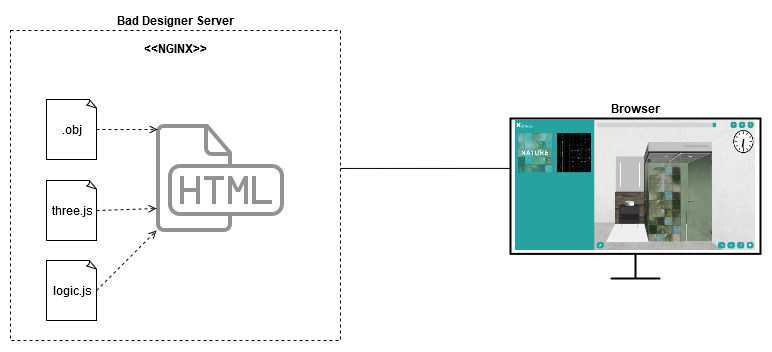
\includegraphics[scale=.3]{images/DA-SysArch.jpg}
    \caption{Systemarchitektur der Web-Applikation}
\end{figure}


\section{Systemarchitektur – Electron Anwendung}

\section*{Erklärung}
Das Electron Executable muss lediglich vom Server heruntergeladen werden und installiert werden. Danach ist die Anwendung sofort einsetzbar. Dadurch das die Applikation mit Electron \ref{sec:Electron} gemacht wurde lässt sie sich wie eine normale Desktopanwendung starten ohne Browser.

\section*{Deployment}
Um die Diplomarbeit als Electron Anwendung zu deployen und benützen muss man lediglich die bestehende Web-App in eine Electron App konvertieren und auf dem Server zum Herunterladen stellen.

\chapter{Zusammenfassung}
Im Laufe der Arbeit sind einige Probleme aufgetreten, die zwar nicht unmöglich zu lösen waren, aber trotzdem nach zeitintensiven Lösungen verlangten. Anfänglich war der Bad-Designer, wegen eines Missverständnisses, ein Konfigurator. Erst nach dem zweiten Gespräch mit dem Auftraggeber wurde der Irrtum ausgebessert. Dank der Flexibilität von Three.js [\ref{sec:three.js}] ist die Umstellung auf die aktuelle Version schnell vorangegangen. Dadurch dass die Dateien mit den Modellen von den Badezimmermodulen immer größer wurden, litt die Performance beim Laden der Website darunter. Dies wurde durch Komprimieren und Umstieg auf einen effizienteren Dateityp behoben, des Weiteren werden die Objekte lokal im Cache gespeichert sobald die Webseite einmal geladen wurde, dass führt noch einmal zu einer Verbesserung der Ladezeit. Den endgültigen Perfomance Schub brachte der Dateityp GLB [\ref{sec:GLB}] und der Draco-Loader [\ref{dracoloader}]. Dadurch dass, der Bad-Designer sowohl als Web-Anwendung als auch als Electron Anwendung [\ref{sec:Electron}] angeboten wird, kann man das Programm lokal und ohne Internet benutzen um eine gewisse Unabhängigkeit zu schaffen.Für das Deployment der Diplomarbeit kam Docker [\ref{sec:Docker}] ins Spiel, durch diese Containervirtualisierung kann die Applikation in kürzester Zeit zur Verfügung gestellt werden. \\
Trotz aller Hürden ist die Diplomarbeit gelungen und der Auftraggeber, \\die {\projectpartner}, mit dem Ergebnis zufrieden. Die Ziele die gesetzt wurden, wurden auch erreicht.


\bibliography{da_bibliography}{}
\bibliographystyle{alphaurl} % alternatives plainurl, alphaurl;  german alternative: dinat (but add package natbib)

\listoffigures
\listoftables
\chapter*{Project Log Book}
\begin{tabular}{|l|l|l|l|}
\hline
Date & Participants & Todos & Due\\
\hline
\end{tabular}

\appendix
\chapter{Additional Information} \label{cha:additional-information}
If needed the appendix is the place where additional information concerning your thesis goes. Examples could be:
\begin{itemize}
	\item Source Code
	\item Test Protocols
	\item Project Proposal
	\item Project Plan
	\item Individual Goals
	\item \ldots
\end{itemize}
Again this has to be aligned with the supervisor.
\chapter{Individual Goals} \label{cha:individual-goals}
This is just another example to show what content could go into the appendix.
\end{document}  